\documentclass[12pt]{memoir}

\def\nsemestre {II}
\def\nterm {Fall}
\def\nyear {2024}
\def\nprofesor {Maria Gillespie}
\def\nsigla {MATH601}
\def\nsiglahead {Advanced Combinatorics}
\def\nlang {ENG}
%\def\darktheme{}
\input{../../headerVarillyDiff}
\usepackage[enableskew]{youngtab}

\begin{document}
%\clearpage
\maketitle
%\thispagestyle{empty}
{\small 
\setlength{\parindent}{0em}
\setlength{\parskip}{1em}

This course will focus on the combinatorics of Young tableaux, crystal bases, root systems, Dynkin diagrams, and symmetric functions arising in representation theory of matrix groups and Lie algebras.

\subsubsection*{Requirements}
Familiarity with the basics of group theory and symmetric functions is helpful.
}
\newpage
\tableofcontents
%\begin{multicols}{2}
\chapter{}

\section{Day 1|20240819}

We will start by reviewing the representation theory of finite groups and the Lie group and Lie algebra representations. The objective is to classify semi-simple Lie algebras and groups. This classification is quite combinatorial. 

\subsection{Review of representation theory of finite groups}

Recall groups are sets $G$ endowed with a binary operation $\circ$ such that 
\begin{enumerate}
    \item There is an identity element $e$: $g\circ e=e\circ g=g$.
    \item Every element possesses an inverse. For each $g$, there is an $h$ such that $g\circ h=e=h\circ g$.
    \item The operation $\circ$ is associative.
\end{enumerate}

\begin{Ex}
    The \term{symmetric group} is the set of permutations of $\bonj{n}$. We denote it $(S_n,\circ)$ where our operation is composition. We will use this group quite a lot.
\end{Ex}

\begin{Ex}
We will be working with $\rGL_n(\bC)$ where $\bC$ will come in as more useful than $\bR$. The \term{general linear group} is characterized by the property that $\det(A)\neq 0$ for $A\in\rGL_n(\bC)$.
\end{Ex}

\begin{Ex}
    Given two groups we can construct $G\x H$ by doing operations pointwise. We can also take subgroups and quotient groups. 
\end{Ex}

\begin{Ex}
    Take the \term{special linear group} $\rSL_n(\bC)$ which is the set of matrices $A$ with $\det(A)=1$. This is a subgroup of $\rGL_n(\bC)$.
\end{Ex}

There's a lot more of matrix groups such as $\rSO_n(\bC)$, $\rSp_{2n}(\bC)$ and unitary groups $\rSU_n(\bC)$. 

\subsubsection{Groups which are representations of themselves}

Symmetry groups are groups of linear transformations of $\bC^n$ (some Euclidean space) that fix some shape. Any such group is a subgroup of $\rGL_n(\bC)$. Matrices here don't collapse points nor anything.

\begin{Ex}
    The symmetry group of a diamond in the plane can be found by analyzing the symmetries of the figure.\red{HMMM}
    The group in question is the Klein-4 group which can be seen as 
    $$\set{\id,r_x,r_y,r_xr_y}.$$
    Similarly we can see it as 
    $$\set{\id,(24),(13),(13)(24)}$$
\end{Ex}

\red{Fell asleep}

\section{Day 2|20240821}

We were looking at direct sums of representations. Recall representations are maps which take group elements to matrices. 

$$\rho\oplus\sg\:G\to\rGL_{n+m}(\bC)$$

and this map will send $g$ to a block matrix. A central question in representation theory is to classify the irreducible representations of some object. This is a central question because for finite groups, irreducible is the same as indecomposable.

\begin{Def}
A representation is \term{indecomposable} when it can't be written as a direct sum of smaller representations.
\end{Def}

Irreducible means that it has no non-trivial proper representations. This is analogous to the idea of prime and irreducible numbers. In the most general case where groups may be infinite, irreducible implies indecomposable. 

\subsection{Alternative definitions for representations}

We may define it as a vector space $V$ with an action $G\x V\to V$ so that
$$g(hv)=(gh)v$$
and it should be a linear action in the sense that $v\mapsto gv$ is a linear transformation.\par 

This is equivalent to the previous definition because $V$ can be seen as $\bC^n$. So the definition gives rise to a map 
$$G\to\Aut(V),\ g\mapsto g\.$$
Even more \emph{objecty} is the next definition. We can see a representation as a module over a group ring $\bC G$. This set is made up of formal linear combinations of elements of $G$.\par 
We endow it with a module structure, for any element $g\in G$ in particular in $\bC G$ we can make it a coefficient $gv\in V$ as a $\bC G$-module.

\subsection{Subrepresentations}

Now that we have all the algebraic structure we can use it to define subrepresentations. Because a subrepresentation will be a subspace which inherits the action for example. 

\begin{Def}
    $W\subseteq V$ is a \term{subrepresentation} of $G$ (when $V$ represents $G$) if 
    \begin{itemize}
        \item $W$ is a subspace of $V$, and
        \item $W$ is $G$-invariant in the sense that the image of $G\x W\to V$ is contained in $W$.
    \end{itemize}
    We will also say that $V$ is \term{irreducible} if there's no proper nonzero subrepresentation $W\subseteq V$.
\end{Def}

Sometimes it is possible to decompose a representation into a direct sum of subrepresentations.

\red{fell asleep}

\begin{Def}
    A \term{character} of a representation is the trace map $g\mapsto\tr(\rho(g))$.
\end{Def}

\textbf{Properties}
\begin{enumerate}
    \item $\chi_{V\oplus W}=\chi_V+\chi_W$. 
    \item $\chi_{V\ox W}=\chi_V\chi_W$.
    \item $\chi_V$ uniquely determines the representation.
\end{enumerate}

\section{Day 3|20240823}

\subsection{Lie groups}

\begin{Def}
    A \term{Lie group} is a real smooth manifold $G$ with a group structure such that 
    $$(g,h)\mapsto gh^{-1}$$
    is differentiable.
\end{Def}

A manifold is a set such that around each point there's a local neighborhood that's topologically equivalent to $\bR^n$. Elliptic curves are examples of manifolds.

\begin{Def}
    An \term{algebraic group} is an algebraic variety with a group structure. In this case the multiplication map should be algebraic.
\end{Def}

In certain specializations these two are the same object. In the case of complex Lie groups, we talk about smooth complex manifolds.

\begin{Ex}
    \begin{itemize}
        \item $(\bC^n,+)$ is a Lie group. But it's not compact. \red{sleepy sleepy}
        \item $\rGL_n$
    \end{itemize}
\end{Ex}

\begin{Lem}
(Zariski-)Closed subgroups of a Lie group are also Lie groups.
\end{Lem}

\begin{Ex}
    In particular $B_n$, the set of upper triangular matrices in $\rGL_n$, forms a Lie group. The torus $T_n$, the group of diagonal matrices, is also a Lie group.\par 
    It is called the torus because it's isomorphic to $(\bC\less0)^n$ and $\bC\less 0$ looks like a circle while $(\bC\less 0)^2$ is the product of two circles which is the torus.
\end{Ex}

\subsubsection{The Classical Groups}

The special linear group $\rSL_n$ consists of matrices whose determinant is 1. The classical groups are called clasiccal because they have very nice properties. In particular type $A$ is what we call $\rSL_n$.\par 
To talk about the special orthogonal group $\rSO_n$ we should first fix a symmetric bilinear form $(\.,\.)$ which is positive-definite. The \term{orthogonal group} $\rO_n$ consists of matrices which preserve this form. The special orthogonal group in particular is the subgroup of matrices with determinant $1$.

\begin{Rmk}
Over $\bR$, $\rO_n$ is actually the group of rigid transformations which is generated by reflections and rotations. For $\rSO_n$, it's only the rotations group.
\end{Rmk}

We can also alternatively define $\rO_n$ as 
$$\set{A\: A^\sT A=I}$$
because 
$$\bra{Av}\ket{Aw}=\bra{v}\ket{w}$$
and from this 
$$v^\sT A^\sT Aw=v^\sT w.$$
Comparing entry by entry we get the desired property.\par 
It's also a fact that $\rO_n$ is disconnected, one component is $\rSO_n$ and the other is the set of matrices with determinant $-1$. Finally \term{type B} means $\rSO_{\text{odd}}$ while $D$ means $\rSO_{\text{even}}$. The type $C$ groups are the symplectic groups.

\section{Day 4|20240826}

Continuing on with the classical groups, we will be talking about the \term{Symplectic group} of even dimension. We will be fixing a symplectic form which is a non-degenerate, skew-symmetric, bilinear form.

\begin{Ex}
    The dot product is not symplectic because it's symmetric.
\end{Ex}

\begin{Ex}
    Consider the form 
    $$v_1w_{2n}+v_2w_{2n-1}+\dots+v_nw_{n+1}-v_{n-1}w_n-v_{n+1}w_{n}-v_{n+2}w_{n-1}-\dots-v_{2n}w_{1}.$$
    If $\Om$ is such a matrix of a form, for example when $2n=6$ we have 
    $$
    \Om\defeq
    \begin{pmatrix}
        &&&&&1\\
        &&&&1&\\
        &&&1&&\\
        &&-1&&&\\
        &-1&&&&\\
        -1&&&&&
    \end{pmatrix}
    \To (v,w)=v^{\sT}\Om w
    $$
\end{Ex}

From this our first definition of the symplectic group is matrices which preserve this product. 

\begin{Def}
    The symplectic group $\rSp_{2n}$ is 
    $$\set{M\:(Mv,Mw)=(v,w)}$$
    or equivalently
    $$\set{M\: M^{\sT}\Om M=\Om}.$$
    We will simplify the notation to type $C$.
\end{Def}

\subsection{Representation of Lie groups}

\begin{Def}
    A representation of a Lie group is a map 
which is also differentiable and a group homomorphism.
\end{Def}

\section{Day 5|20240828}

For a partition $\la\vdash n$, we call $S^\la V$
$$\La^{\mu_1}V\ox\La^{\mu_2}V\oxyox\La^{\mu_k}V$$
where $\mu$ is the conjugate partition. 

\begin{Ex}
    For example if $\la=(5,4,1)$, then $\mu=(3,2,2,2,1)$ and so 
    $$S^{(5,4,1)}V=\La^3$$
    Elements can be written as a filling to the Young diagram. Such an element could be 
    $$(v_1\land v_2\land v_3)\ox(a\land b)\ox (c\land d)\ox (x\land y)\ox z$$
    and filling the diagram we have
    $$
    \young(r,qbdy,pacxz).
$$
It's important to familiarize ourselves with this idea so we will itechangebly talk about 
$$(e_1\w e_4\w e_3)\ox(e_1\w e_2)\ox (e_5\w e_3)\ox(e_2\w e_1)\ox e_2$$
and 
$$\young(3,4231,11522)=-\young(4,3231,11522)$$
The tableau $\young(1,12)$ is zero for example.
\end{Ex}

For a basis of $S^\la$, we can talk about it being spanned by elementary tableau where we order each column from least to greatest. These are called \term{column-strict tableau}. For example

$$\young(6,453,1212)$$

If $V$ is an $n$-dimensional vector space, then we have a largest element on our basis. This allows us to formulate the question:
\begin{significant}
How many column strict tableau are there with largest entry $n$? And shape $\la$.
\end{significant}
From this 
$$\binom{n}{\mu_1}\binom{n}{\mu_2}\dots\binom{n}{\mu_k}=S^\la V.$$

\begin{Def}
    The \term{Schur module} $V^\la$ is 
    $$V^\la=\quot{S^\la}{\genr{v_T-\sum_S v_S}}$$
    where the sum is over $S$'s obtained from $T$ by
    \begin{enumerate}
        \item Choose two columns of $C_1,C_2$ of $T$.
        \item Choose $k$ elements from $C_2$.
        \item Exchange them with $k$ elements from $C_1$ in all ways that preserve the order of the elements.
    \end{enumerate}
\end{Def}

\begin{Ex}
    Take $(4,3,3)$ with the filling 
    $$\young(576,244,1134)$$
    so choose the first and third columns as $C_1$ and $C_2$. One relation in $V_\la$
\end{Ex}

\begin{Th}
    The collection 
    $$\set{e_T\:\ T \text{semistandard} \sh(T)\vdash n}$$
    is a basis for the Schur module.
\end{Th}

\section{Day 6|20240830}

Last time we defined the Schur modules. These are 

$$S^\la V=\La^{\mu_1}V\oxyox \La^{\mu_r}$$

where $\mu=\la^\ast$ is the conjugate or transpose. Now $V^\la$ is $S^\la$ modded out by column exchanges. We will show that 
$$\set{e_T\: T\in SSYT(\la), \text{largest entry}\leq n}$$
is a basis for $V^\la$.

\begin{Ex}
    Consider the tableau
    $$\young(6,53,214)$$
    the second and third row are wrongfully ordered
\end{Ex}

\red{Sleepy sleepy}

We wil show that they are independent in the quotient. 

\begin{Ex}
    The idea for why $D_T$'s are independent. We can find lex orderings and make $D_T$ have nice leading term and then an ordering on the leading terms. E.g. $1,1+x,1+x+x^2,1+x+x^2+x^3$ are independent because the leading terms are all distinct.\par 
    In $V^{\young(a,bc)}$ we have 
    $$D_{\young(2,11)}=\det\twobytwo{z_{11}}{z_{12}}{z_{21}}{z_{22}}z_{11}=\dots$$
    And 
    $$D_{\young(2,12)}=z_{12}\det$$
    In the monomials $z_{11}^2z_{22}$ is larger than $z_{11}z_{12}z_{22}$ and that's how we show that they're independent of each other. This shows the elementary symmetric functions are independent. 
\end{Ex}

One exciting conclusion to look at it's characters. For a Lie group the right notion is to consider $H$ a maximal torus in a Lie group $G$. This is the maximal connecated, abelian Lie sub group.

\begin{Ex}
    $T_n\subseteq\rGL_n$ in this case $\chi_V\: H\to \bC$ where $h\mapsto\tr(h\text{ acts on } V)$. This $\chi_V$ determines $V$ and has nice properties with direct sum and tensor products.
    $$\chi_V\diag(x_1,\dots,x_n)$$
    is the trace of that matrix acting on $V^\la$. It suffices to look at a basis. For a given $e_T$ where $T$ is a SSYT, $X$ acts on each $e_i$ by doing $x_ie_i$. see
    $$\young(3,234,112)=x_1x_1x_2x_2x_3x_3x_4\.\young(3,234,112)$$
    now the trace is the sum of the eigenvalues and this is $x^T$. So 
    $$\sum_{T SSYT}x^T=s_\la(\un x).$$
\end{Ex}

\section{Day 7|20240904}

\begin{Th}
A representation of $\rGL_n$ is irreducible if and only if it has a unique highest weight vector.
\end{Th}

\begin{Def}
    A \term{weight vector} of $V$ is $v\in V$ such that for $x\in T_n$ (the torus), 
    $$x\.v=x_1^{\al_1}\dots x_n^{\al_n}v$$
    where $\al=(\al_1,\dots,\al_n)\in\bZ^n$ is weight.
\end{Def}

Recall that being in the torus meant $x=\threebythree{x_1}{\dots}{0}{\vdots}{\ddots}{\vdots}{0}{\dots}{x_n}$.

\begin{Def}
    A \term{highest weight vector} is a weight vector such that 
    $$B_n\.v=\bC^\ast\. v$$
    where $B_n$ is the Borel matrices compromised of upper triangular matrices.
\end{Def}

A representation is a sum of its weights: $V=\bigoplus_{\al}V_\al$ where $V_\al=\set{v\:\ x\.dot v=x^\al v}$.

\begin{Lem}
The only highest weight vector in $V^\la$ is $e_{T_0}$ where $T_E$
\end{Lem}

\section{Day n|20240930}

\subsection{Combinatorics of $\gsl_3$ representations}

Our goal for today is to see how all irreducible $\gsl_3$ representations live in $(V^{(1,0)})^{\ox n}$. We would like to describe them. Recall $V^{(1,0)}$ means that we have $1L_1$ and no $L_2$.\par
As a shorthand we will say 
$$F_1=F_{12}, F_2=F_{23}, E_1=E_{12},\dots$$

\begin{Def}
    The word $a_1\dots a_n\in\set{1,2,3}^n$ represents the weight space corresponding to the $L$-diagram calculation in $(V^{(1,0)})^{\ox n}$ corresponding to 
    $a_1\oxyox a_n$.
\end{Def}

\begin{Lem}
    The weight of $(a_1\dots a_n)$ is $(\# 1's,\# 2's,\# 3's)$.
\end{Lem}

\begin{ptcbp}
By induction on $n$, the base case is a diagram. \red{ASK FOR DIAGRAM,}. Then the induction step wishes to show that \red{something} is additivw across $\ox$. So recall, ¿why are weights additive across $\ox$? Let $v_\al,v_\bt$ be weight vectors. We want to show $\al,\bt\in\eta^\ast=\set{H\to\bC}$. Then \red{finish}
\end{ptcbp}

\begin{Cor}
The highest weight words in $(V^{(1,0)})^{\ox n}$ are $a_1\dots a_n$ such that very suffix  has $(\#1's)\geq(\#2's)\geq(\#3's)$.
\end{Cor}

The proof is basically noting that $E_1,E_2$ map the word to zero when it's of highest weight.

\begin{Ex}
    $(V^{(1,0)})^{\ox 3}$ so first we find the heighest weight words: $111,121,211$ and $321$. 
    \begin{figure}
        
\tikzset{every picture/.style={line width=0.75pt}} %set default line width to 0.75pt        

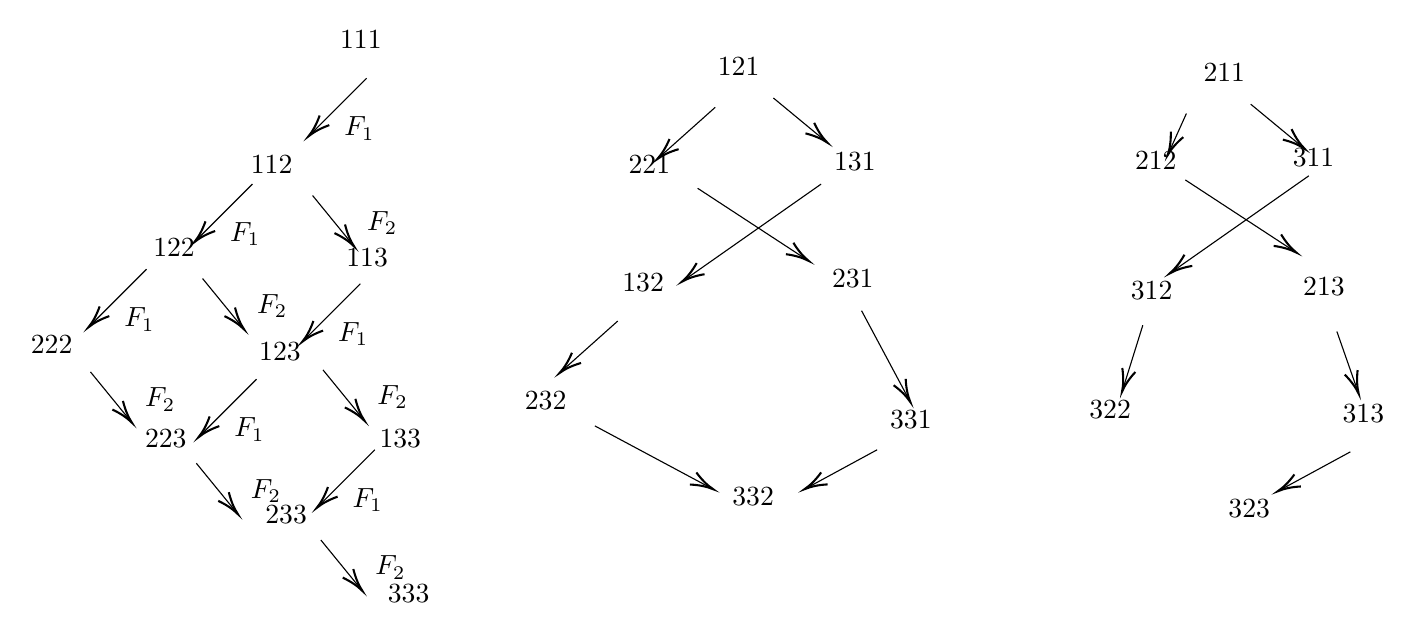
\begin{tikzpicture}[x=0.75pt,y=0.75pt,yscale=-1,xscale=1]
%uncomment if require: \path (0,300); %set diagram left start at 0, and has height of 300

%Straight Lines [id:da42089973349634247] 
\draw    (179,27.5) -- (152.41,54.09) ;
\draw [shift={(151,55.5)}, rotate = 315] [color={rgb, 255:red, 0; green, 0; blue, 0 }  ][line width=0.75]    (10.93,-3.29) .. controls (6.95,-1.4) and (3.31,-0.3) .. (0,0) .. controls (3.31,0.3) and (6.95,1.4) .. (10.93,3.29)   ;
%Straight Lines [id:da3031105581540732] 
\draw    (176,126.5) -- (149.41,153.09) ;
\draw [shift={(148,154.5)}, rotate = 315] [color={rgb, 255:red, 0; green, 0; blue, 0 }  ][line width=0.75]    (10.93,-3.29) .. controls (6.95,-1.4) and (3.31,-0.3) .. (0,0) .. controls (3.31,0.3) and (6.95,1.4) .. (10.93,3.29)   ;
%Straight Lines [id:da803008915658254] 
\draw    (124,78.5) -- (97.41,105.09) ;
\draw [shift={(96,106.5)}, rotate = 315] [color={rgb, 255:red, 0; green, 0; blue, 0 }  ][line width=0.75]    (10.93,-3.29) .. controls (6.95,-1.4) and (3.31,-0.3) .. (0,0) .. controls (3.31,0.3) and (6.95,1.4) .. (10.93,3.29)   ;
%Straight Lines [id:da8767210663804941] 
\draw    (73,119.5) -- (46.41,146.09) ;
\draw [shift={(45,147.5)}, rotate = 315] [color={rgb, 255:red, 0; green, 0; blue, 0 }  ][line width=0.75]    (10.93,-3.29) .. controls (6.95,-1.4) and (3.31,-0.3) .. (0,0) .. controls (3.31,0.3) and (6.95,1.4) .. (10.93,3.29)   ;
%Straight Lines [id:da11711889811973819] 
\draw    (126,172.5) -- (99.41,199.09) ;
\draw [shift={(98,200.5)}, rotate = 315] [color={rgb, 255:red, 0; green, 0; blue, 0 }  ][line width=0.75]    (10.93,-3.29) .. controls (6.95,-1.4) and (3.31,-0.3) .. (0,0) .. controls (3.31,0.3) and (6.95,1.4) .. (10.93,3.29)   ;
%Straight Lines [id:da5343444040412961] 
\draw    (183,206.5) -- (156.41,233.09) ;
\draw [shift={(155,234.5)}, rotate = 315] [color={rgb, 255:red, 0; green, 0; blue, 0 }  ][line width=0.75]    (10.93,-3.29) .. controls (6.95,-1.4) and (3.31,-0.3) .. (0,0) .. controls (3.31,0.3) and (6.95,1.4) .. (10.93,3.29)   ;
%Straight Lines [id:da8170158271849678] 
\draw    (153,84) -- (171.74,106.95) ;
\draw [shift={(173,108.5)}, rotate = 230.77] [color={rgb, 255:red, 0; green, 0; blue, 0 }  ][line width=0.75]    (10.93,-3.29) .. controls (6.95,-1.4) and (3.31,-0.3) .. (0,0) .. controls (3.31,0.3) and (6.95,1.4) .. (10.93,3.29)   ;
%Straight Lines [id:da2307297886745664] 
\draw    (100,124) -- (118.74,146.95) ;
\draw [shift={(120,148.5)}, rotate = 230.77] [color={rgb, 255:red, 0; green, 0; blue, 0 }  ][line width=0.75]    (10.93,-3.29) .. controls (6.95,-1.4) and (3.31,-0.3) .. (0,0) .. controls (3.31,0.3) and (6.95,1.4) .. (10.93,3.29)   ;
%Straight Lines [id:da7984622676548068] 
\draw    (46,169) -- (64.74,191.95) ;
\draw [shift={(66,193.5)}, rotate = 230.77] [color={rgb, 255:red, 0; green, 0; blue, 0 }  ][line width=0.75]    (10.93,-3.29) .. controls (6.95,-1.4) and (3.31,-0.3) .. (0,0) .. controls (3.31,0.3) and (6.95,1.4) .. (10.93,3.29)   ;
%Straight Lines [id:da5520008445276355] 
\draw    (158,168) -- (176.74,190.95) ;
\draw [shift={(178,192.5)}, rotate = 230.77] [color={rgb, 255:red, 0; green, 0; blue, 0 }  ][line width=0.75]    (10.93,-3.29) .. controls (6.95,-1.4) and (3.31,-0.3) .. (0,0) .. controls (3.31,0.3) and (6.95,1.4) .. (10.93,3.29)   ;
%Straight Lines [id:da1625762686635499] 
\draw    (97,213) -- (115.74,235.95) ;
\draw [shift={(117,237.5)}, rotate = 230.77] [color={rgb, 255:red, 0; green, 0; blue, 0 }  ][line width=0.75]    (10.93,-3.29) .. controls (6.95,-1.4) and (3.31,-0.3) .. (0,0) .. controls (3.31,0.3) and (6.95,1.4) .. (10.93,3.29)   ;
%Straight Lines [id:da1026725922353392] 
\draw    (157,250) -- (175.74,272.95) ;
\draw [shift={(177,274.5)}, rotate = 230.77] [color={rgb, 255:red, 0; green, 0; blue, 0 }  ][line width=0.75]    (10.93,-3.29) .. controls (6.95,-1.4) and (3.31,-0.3) .. (0,0) .. controls (3.31,0.3) and (6.95,1.4) .. (10.93,3.29)   ;
%Straight Lines [id:da4681112463331931] 
\draw    (375,37) -- (399.46,57.23) ;
\draw [shift={(401,58.5)}, rotate = 219.59] [color={rgb, 255:red, 0; green, 0; blue, 0 }  ][line width=0.75]    (10.93,-3.29) .. controls (6.95,-1.4) and (3.31,-0.3) .. (0,0) .. controls (3.31,0.3) and (6.95,1.4) .. (10.93,3.29)   ;
%Straight Lines [id:da657993683720376] 
\draw    (347,41.5) -- (320.49,65.17) ;
\draw [shift={(319,66.5)}, rotate = 318.24] [color={rgb, 255:red, 0; green, 0; blue, 0 }  ][line width=0.75]    (10.93,-3.29) .. controls (6.95,-1.4) and (3.31,-0.3) .. (0,0) .. controls (3.31,0.3) and (6.95,1.4) .. (10.93,3.29)   ;
%Straight Lines [id:da23694615966603938] 
\draw    (398,78.5) -- (332.64,124.35) ;
\draw [shift={(331,125.5)}, rotate = 324.95] [color={rgb, 255:red, 0; green, 0; blue, 0 }  ][line width=0.75]    (10.93,-3.29) .. controls (6.95,-1.4) and (3.31,-0.3) .. (0,0) .. controls (3.31,0.3) and (6.95,1.4) .. (10.93,3.29)   ;
%Straight Lines [id:da6217535822776135] 
\draw    (338.5,80.5) -- (390.33,114.41) ;
\draw [shift={(392,115.5)}, rotate = 213.19] [color={rgb, 255:red, 0; green, 0; blue, 0 }  ][line width=0.75]    (10.93,-3.29) .. controls (6.95,-1.4) and (3.31,-0.3) .. (0,0) .. controls (3.31,0.3) and (6.95,1.4) .. (10.93,3.29)   ;
%Straight Lines [id:da6082139480648872] 
\draw    (300,144.5) -- (273.49,168.17) ;
\draw [shift={(272,169.5)}, rotate = 318.24] [color={rgb, 255:red, 0; green, 0; blue, 0 }  ][line width=0.75]    (10.93,-3.29) .. controls (6.95,-1.4) and (3.31,-0.3) .. (0,0) .. controls (3.31,0.3) and (6.95,1.4) .. (10.93,3.29)   ;
%Straight Lines [id:da3195984051533788] 
\draw    (289,195) -- (344.24,224.56) ;
\draw [shift={(346,225.5)}, rotate = 208.15] [color={rgb, 255:red, 0; green, 0; blue, 0 }  ][line width=0.75]    (10.93,-3.29) .. controls (6.95,-1.4) and (3.31,-0.3) .. (0,0) .. controls (3.31,0.3) and (6.95,1.4) .. (10.93,3.29)   ;
%Straight Lines [id:da6108309460864101] 
\draw    (425,206.5) -- (391.76,224.55) ;
\draw [shift={(390,225.5)}, rotate = 331.5] [color={rgb, 255:red, 0; green, 0; blue, 0 }  ][line width=0.75]    (10.93,-3.29) .. controls (6.95,-1.4) and (3.31,-0.3) .. (0,0) .. controls (3.31,0.3) and (6.95,1.4) .. (10.93,3.29)   ;
%Straight Lines [id:da2663257070875219] 
\draw    (417.5,139.5) -- (440.06,181.74) ;
\draw [shift={(441,183.5)}, rotate = 241.89] [color={rgb, 255:red, 0; green, 0; blue, 0 }  ][line width=0.75]    (10.93,-3.29) .. controls (6.95,-1.4) and (3.31,-0.3) .. (0,0) .. controls (3.31,0.3) and (6.95,1.4) .. (10.93,3.29)   ;
%Straight Lines [id:da41104506477492275] 
\draw    (605,40) -- (612.56,46.25) -- (629.46,60.23) ;
\draw [shift={(631,61.5)}, rotate = 219.59] [color={rgb, 255:red, 0; green, 0; blue, 0 }  ][line width=0.75]    (10.93,-3.29) .. controls (6.95,-1.4) and (3.31,-0.3) .. (0,0) .. controls (3.31,0.3) and (6.95,1.4) .. (10.93,3.29)   ;
%Straight Lines [id:da3109726409881449] 
\draw    (574,44.5) -- (565.82,62.68) ;
\draw [shift={(565,64.5)}, rotate = 294.23] [color={rgb, 255:red, 0; green, 0; blue, 0 }  ][line width=0.75]    (10.93,-3.29) .. controls (6.95,-1.4) and (3.31,-0.3) .. (0,0) .. controls (3.31,0.3) and (6.95,1.4) .. (10.93,3.29)   ;
%Straight Lines [id:da4421494524769354] 
\draw    (633,74.5) -- (567.64,120.35) ;
\draw [shift={(566,121.5)}, rotate = 324.95] [color={rgb, 255:red, 0; green, 0; blue, 0 }  ][line width=0.75]    (10.93,-3.29) .. controls (6.95,-1.4) and (3.31,-0.3) .. (0,0) .. controls (3.31,0.3) and (6.95,1.4) .. (10.93,3.29)   ;
%Straight Lines [id:da32714587117225613] 
\draw    (573.5,76.5) -- (625.33,110.41) ;
\draw [shift={(627,111.5)}, rotate = 213.19] [color={rgb, 255:red, 0; green, 0; blue, 0 }  ][line width=0.75]    (10.93,-3.29) .. controls (6.95,-1.4) and (3.31,-0.3) .. (0,0) .. controls (3.31,0.3) and (6.95,1.4) .. (10.93,3.29)   ;
%Straight Lines [id:da203922877186004] 
\draw    (553,146.5) -- (543.6,176.59) ;
\draw [shift={(543,178.5)}, rotate = 287.35] [color={rgb, 255:red, 0; green, 0; blue, 0 }  ][line width=0.75]    (10.93,-3.29) .. controls (6.95,-1.4) and (3.31,-0.3) .. (0,0) .. controls (3.31,0.3) and (6.95,1.4) .. (10.93,3.29)   ;
%Straight Lines [id:da4533498811545599] 
\draw    (646.5,149.5) -- (656.34,177.61) ;
\draw [shift={(657,179.5)}, rotate = 250.71] [color={rgb, 255:red, 0; green, 0; blue, 0 }  ][line width=0.75]    (10.93,-3.29) .. controls (6.95,-1.4) and (3.31,-0.3) .. (0,0) .. controls (3.31,0.3) and (6.95,1.4) .. (10.93,3.29)   ;
%Straight Lines [id:da31860421298697295] 
\draw    (653,207.5) -- (619.76,225.55) ;
\draw [shift={(618,226.5)}, rotate = 331.5] [color={rgb, 255:red, 0; green, 0; blue, 0 }  ][line width=0.75]    (10.93,-3.29) .. controls (6.95,-1.4) and (3.31,-0.3) .. (0,0) .. controls (3.31,0.3) and (6.95,1.4) .. (10.93,3.29)   ;

% Text Node
\draw (165,3.4) node [anchor=north west][inner sep=0.75pt]    {$111$};
% Text Node
\draw (122,63.4) node [anchor=north west][inner sep=0.75pt]    {$112$};
% Text Node
\draw (168,108.4) node [anchor=north west][inner sep=0.75pt]    {$113$};
% Text Node
\draw (126,153.4) node [anchor=north west][inner sep=0.75pt]    {$123$};
% Text Node
\draw (75,103.4) node [anchor=north west][inner sep=0.75pt]    {$122$};
% Text Node
\draw (16,150.4) node [anchor=north west][inner sep=0.75pt]    {$222$};
% Text Node
\draw (71,195.4) node [anchor=north west][inner sep=0.75pt]    {$223$};
% Text Node
\draw (184,195.4) node [anchor=north west][inner sep=0.75pt]    {$133$};
% Text Node
\draw (129,232.4) node [anchor=north west][inner sep=0.75pt]    {$233$};
% Text Node
\draw (188,270.4) node [anchor=north west][inner sep=0.75pt]    {$333$};
% Text Node
\draw (167,44.9) node [anchor=north west][inner sep=0.75pt]    {$F_{1}$};
% Text Node
\draw (164,143.9) node [anchor=north west][inner sep=0.75pt]    {$F_{1}$};
% Text Node
\draw (112,95.9) node [anchor=north west][inner sep=0.75pt]    {$F_{1}$};
% Text Node
\draw (61,136.9) node [anchor=north west][inner sep=0.75pt]    {$F_{1}$};
% Text Node
\draw (114,189.9) node [anchor=north west][inner sep=0.75pt]    {$F_{1}$};
% Text Node
\draw (171,223.9) node [anchor=north west][inner sep=0.75pt]    {$F_{1}$};
% Text Node
\draw (178,104.1) node [anchor=south west] [inner sep=0.75pt]    {$F_{2}$};
% Text Node
\draw (125,144.1) node [anchor=south west] [inner sep=0.75pt]    {$F_{2}$};
% Text Node
\draw (71,189.1) node [anchor=south west] [inner sep=0.75pt]    {$F_{2}$};
% Text Node
\draw (183,188.1) node [anchor=south west] [inner sep=0.75pt]    {$F_{2}$};
% Text Node
\draw (122,233.1) node [anchor=south west] [inner sep=0.75pt]    {$F_{2}$};
% Text Node
\draw (182,270.1) node [anchor=south west] [inner sep=0.75pt]    {$F_{2}$};
% Text Node
\draw (347,16.4) node [anchor=north west][inner sep=0.75pt]    {$121$};
% Text Node
\draw (403,61.9) node [anchor=north west][inner sep=0.75pt]    {$131$};
% Text Node
\draw (304,63.4) node [anchor=north west][inner sep=0.75pt]    {$221$};
% Text Node
\draw (301,120.4) node [anchor=north west][inner sep=0.75pt]    {$132$};
% Text Node
\draw (402,118.4) node [anchor=north west][inner sep=0.75pt]    {$231$};
% Text Node
\draw (254,177.4) node [anchor=north west][inner sep=0.75pt]    {$232$};
% Text Node
\draw (581,19.4) node [anchor=north west][inner sep=0.75pt]    {$211$};
% Text Node
\draw (548,61.4) node [anchor=north west][inner sep=0.75pt]    {$212$};
% Text Node
\draw (624,60.4) node [anchor=north west][inner sep=0.75pt]    {$311$};
% Text Node
\draw (546,124.4) node [anchor=north west][inner sep=0.75pt]    {$312$};
% Text Node
\draw (629,122.4) node [anchor=north west][inner sep=0.75pt]    {$213$};
% Text Node
\draw (526,181.4) node [anchor=north west][inner sep=0.75pt]    {$322$};
% Text Node
\draw (593,229.4) node [anchor=north west][inner sep=0.75pt]    {$323$};
% Text Node
\draw (648,183.4) node [anchor=north west][inner sep=0.75pt]    {$313$};
% Text Node
\draw (354,223.4) node [anchor=north west][inner sep=0.75pt]    {$332$};
% Text Node
\draw (430,186.4) node [anchor=north west][inner sep=0.75pt]    {$331$};


\end{tikzpicture}

    \end{figure}
    So this first one gives us an adjoint representation, the next one also gives us another adjoint. So this last one for $111$ gives us the last 10 elements. The $321$ gives us the last one. From this the representation decomposes as
    $$V^{(3,0)}\oplus(V^{(2,1)})^(\oplus 2)\oplus V^{(0,0)}.$$
    They all have the same weight but are independent one-dimensional weight spaces. Each word on the $111$ diagram has a different weight. How many words have weight $(1,2)$, its $122,212$ and $221$ so the dimesion of that space is $3=\binom{3}{2}=\binom{3}{1}$. 
\end{Ex}

\begin{Qn}
In $(V^{(1,0)})^{\ox n}$, ¿what is the dimension of the weight space $\al=(a,b,c)=(a-c,b-c)$? It's however many words of length $n$ have $a$ $1'$s, $b$ $2'$s and $c$ $3'$s. This is $\binom{n}{a,b,c}=\frac{n!}{a!b!c!}$, which is counted by taking all the words and then dividing by possible rearrangements. This gives us something with the dots in the diagram. 
\end{Qn}

Recall from when we talked about RSK insertion: It is compatible with $\gsl_2$ crystal operations on tableau reading word. In other words this is, if $\un a\xrightarrow{F_i}\un{b}$ then 
\begin{itemize}
    \item The RSK insertion tableau of $\un a,\un b$ matches.
    \item $\rw(\ins(\un a))\xrightarrow{F_i}\rw(\ins(\un b))$.
\end{itemize}

So in conclusion, each connected component (irreducible representation) in $(V^{(1,0)})^{\ox n}$ corresponds to a recording tableau. Let's see how this works: 

\begin{Ex}
    If we take the RSK insertion of the diagram we get \red{diagram}. The bumping sequence is all the same! What that means is that we can take the reading word and apply $F_1$. So all the stuff we did on crystals in 502 is coming back.\par
    If we take the other one for $211$, the RSK insetion is $\young(2,11)$ but the recording tableau is $\young(2,13)$ so we're gonna count how many times an irreducible representation shows up by counting tableau.
\end{Ex}

\section{Day n+1|20241002}

Recall $(V^{(1,0)})^{\ox n}$ is described by words of $1,2,3$ of length $n$ with $F_1,F_2$ bracketing rules.
$E_1,E_2$ also have bracketing rules. Consider the word
$$1223112133212\to)((?))()??()($$
so $E_1$ changes the leftmost unpaired $2$ to a $1$ which leaves us with 
$$1223112133211\to)((?))()??()).$$
The highest weight is the ballot word which when read right to left has more $\#i$'s than $\#i+1$'s.

\begin{Ex}
    We have $(V^{(1,0)})^{\ox 4}$ with dimension $3^4=81$. The highest weight words, or ballot\footnote{Yamanouchi or reverse ballot} words are
    $$1111,1121,1211,1321,2111,2121,2211,3121,3211$$
    corresponding to 
    $$V^{(4,0)},V^{(3,1)},V^{(3,1)},V^{(2,1,1)}=V^{(1,0)},V^{(3,1)},V^{(2,2)},V^{(2,2)},V^{(1,0)},V^{(1,0)}.$$
    So this is 
    $$V^{(4,0)}\oplus (V^{(3,1)})^{\oplus 3}\oplus(V^{(2,2)})^{\oplus 2}\oplus(V^{(1,0)})^{\oplus 3}.$$
\end{Ex}
Recall that $V^{(2,1,1)}=V^{(1,0)}$ because $L_1+L_2+L_3=0$ and we can quotient out by $(1,1,1)$.\par
Let's recall some crystal/Young tableaux facts:
\begin{enumerate}
    \item RSK recording tableau is unchanged via $F_1,F_2$.
    \item Any highest weight word has RSK insertion tableau that looks like 
    $$\young(33,222,1111)$$
    where all $i'$s are in row $i$ from the bottom.
\end{enumerate}
This facts imply that two connected components of $(V^{(1,0)})^{\ox n}$ crystal have different recording tableau as RSK is a bijection.
\begin{Ex}
    We have that 
    $$3121\xrightarrow{RSK}[[3[]]]$$
\end{Ex}

\section{Day n+2| 20241004}

\subsection*{Characters of $\gsl_3$ representations}

The last time we talked about 
$$\chi(V)=\sum_{\al\in\La}\dim(V_\al)x^\al.$$
There's this fact which is the \emph{highest weight theorem} which states:

\begin{Th}
    $V$ is determined by $\chi(V)$.
\end{Th}

The idea of this for $\gsl_3$ is that we had the hexagonal lattice which was generated by a unique highest weight element.\par
So given $\ch(V)$, let $x^\al$ appear in $\ch(V)$ where $\al$ is a highest weight, subtract $\ch(V^\al)$ and iterate.\par
With the notation 
$$x^\al=x_1^{\al_1}x_2^{\al_2}x_3^{\al_3}$$
we ask what is the character of $V^{(a,b)}$?

\begin{Ex}
    We've written $V^{(1,0)}$ as 
    \begin{center}
        FIGURE
    \end{center}
    Summing up the monomials we can see that this is 
    $$\chi(V^{(2,1)})=s_{(2,1)}\bmod x_1x_2x_3.$$
\end{Ex}

\begin{Prop}
The character of $V^{(a,b)}$ is 
$$\chi(V^{(a,b)})=s_{(a,b)}(x_1,x_2,x_3)\bmod x_1x_2x_3.$$
\end{Prop}

This isn't immediately obvious. We have a bunch of words and insert them, but we need to see that every SSYT occurs.

\begin{ptcbp}
    Recall 
    $$s_{(a,b)}(x_1,x_2,x_3)=\sum_{\substack{T\in SSYT(a,b)\\ 1,2,3}}x^T.$$
    We claim that every SSYT T is obtained from a sequence of $F_1,F_2$'s applied to 
    $$\young(222,11111)$$
    We ought to show we can get back to it with $E's$. Let's do this more generally for $\gsl_n$. If $T$ is not highest weight, we will show that we can apply a raising operator.\par
    Let $r$ be the lowest row such that $T$ doesn't have all $r$'s in that row. Say $r=3$ then in 
    $$\young(45,3345,2222,11111)$$
    we take the rightmost element $i$ of row $r$. This means that $i>r$. This is, in this case $i=5$. We may now apply $E_{i-1}$ which is well defined because in row $r$, there's no $i-1$ below it. Here $i-1\geq r$ for all rows below a  $r-1$.
    So bracketing $i,i-1$ there is an upaired $i$ to which we may apply $E_i$.insertion \red{sleep}
\end{ptcbp}

This first Littlewood Richardson rule is concatenate reading words like in $\gsl_2$. The coefficient is 
$$c_{\la\mu}^\nu=\# \text{pairs} (T,S) \text{of shapes }\la,mu(unfinished)$$
The third LR rule is in terms of skew tableau. The LR coefficient is then $\#$ of skew SSYT of shape $\nu/\la$ and content $\mu$ with a ballot reading word. Proving this is harder but it's not so bad when we think of a skew crystal. It's not obvious what's going on. Recall the Hall inner product which gives us 
$$\braket{s_\mu s_\la}{s_\nu}=c_{\la\mu}^\nu=\braket{s_\mu}{s_{\nu/\la}}.$$

\section{Day n+3| 20241007}

\subsection{Representations of $\gsl_n$}

There's no steps of thinking to this. It's the same as $\gsl_3$. Recall $\gsl_n$ corresponds to $n\x n$ matrices which are traceless. The Cartan subalgebra of $\gsl_n$ is 
$$\lie{h}=\set{\text{diagonal matrices }M,\ \tr M=0}.$$
Then elements here are $H=\diag(x_1,\dots,x_n)$ such that $\sum x_i=0$. To define weights, these live in $\lie h^\ast$ and they are joint eigenvalues of $H$ in a representation $V$ of $\gsl_n$. In other words, $\al\in\lie h^\ast$ with $v_\al\in V$ such that 
$$Hv_\al=\al(H)v_\al,\word{for}H\in\lie h.$$

\begin{Ex}
    If $\al\diag(x_1,\dots,x_n)=x_1$ then this is $L_1$. $L_i$ is such that $L_i\diag(\un x)=x_i$.
\end{Ex}

The \term{weight space} is $L_1+\dots+L_n=0$. What are all the weights which are valid for representations? The weight lattice is $\genr{L_1\dots,L_n}$ and all weights lie on the lattice. The proof proceeds the same way, taking block copies of $\gsl_2$.

\subsection{Adjoint representation of $\gsl_n$}

In $\gsl_3$, the adjoint representation had dimension 8.  

\subsection{Crystals for $\gsl_n$}

$(1,0,\dots,0)=L_1$

\begin{Th}
    $(V^{L_1})^{\ox m}=\bigoplus c_\la V^{\la}$
    where $c_\la=\#SYT(\la)$
\end{Th}

The proof is done using crystals and RSK, every connected component corresponds to a unique recording tableau.

\section{Day n+4| 20241009}

\subsection{$\gsl_n$ crystals and Stembridge axioms}

Consider the word 
$$21132342132$$
we claim that the operations $F_1$ and $F_3$ commute in $\gsl_n$. Observe that $F_1$ brackets $(1,2)$ and $F_3$ brackets $(3,4)$. 
We thus get:
\begin{align*}
    &F_1(21132342132)=21232342132\\
    &F_3(21132342132)=21132442132\\
\end{align*} 
and then applying $F_3,F_1$ respectively we get the same word 
$$21232442132.$$
Sometimes $F_1F_3$ is not defined so we actually mean that 
$$F_1F_3(x)=y\To F_3F_1(x)=y$$
even when $y=0$. We have a lot of commuting squares then! We may generalize to 

\begin{Th}
    $F_i,F_j$ commute when $|i-j|>1$. 
\end{Th}

This characterizes the crystal graphs but not completely, that's where the Stembridge axioms come into play. 

\begin{Th}
    In an $\gsl_n$ crystal, for $F_1(w),F_2(w)$ either:
    \begin{enumerate}
        \item $\exists z (z=F_1F_2(w)=F_2F_1(w))$, or
        \item $\exists u,v,s,t,z$ such that the crystal is just like the adjoint representation. This means that 
        $$F_2F_1F_1F_2=F_1F_2F_2F_1.$$
    \end{enumerate}
\end{Th}

¿Why can't we have more complicated words than that? The proof for this will be very combinatorial and we will analyze a lot of words.

\begin{ptcbp}
    Let $a$ be the rightmost unpaired $1$ in $w$ for $(1,2)$. Then call $b$ the rightmost unpaired $2$ in $w$ for $(2,3)$.
    \begin{itemize}
        \item In the first case, we assume that removing $b$ does not unbracket a $1$. Take for example\red{sleep}
        \item In the next case $F_1F_1F_2$
        \item The third case is basically removing $b=2$ unpairs $c=1$, where $b$ is left of $a$ and there exists and unpaired $3$ to the left of $a$. This is 
        $$-2-1-(3)-1-$$
        so applying $F_1$ gets us $-2132-$ and $F_2$ leaves us with $-3131-$. This both meet up after applying $F_2$ and $F_1$ respectively.
        \item Finally it could be like before but there's no unpaired $3$ left of $a$. Here we get another figure 8 diagram. For this case we get 
    \end{itemize}
    

\end{ptcbp}

This all comes from Stembridge's 2004 paper. 

\section{Day n+5|20241011}

We were talking about how the figure 8 and sqaure characterizes stuff. We will now characterize crystals as graphs. 

\subsection{Crystals of type $A$}

\begin{Def}
A type $A$ \term{Kashiwara} crystal of finite type is
\begin{itemize}
    \item $B$ a crystal base (weight spaces' generators are bases), nonempty set.
    \item Two arrow maps $e_i,f_i\: B\to B\cupdot \set{emptyset}$ for $i\in\bonj{n-1}$.
    \item Two length maps $\eps_i,\vf_i\: B\to\bZ$ which correspond to the number of times you can apply $e_i$ and $f_i$.
    \item And a weight function to thw lattice $\wt\: B\to\La$ where $\La\bZ\genr{L_1,\dots,L_n}$ and $\sum L_i=0$. Elements here are $\un a/\un 1$, i.e. modded by translations.
\end{itemize}
They must satisfy the properties
\begin{enumerate}
    \item If $x,y\in B$, then 
    $$e_i(X)=y\iff x=f_i(y)$$
    and in this case
    $$\wt(y)=\wt(x)+\al_i$$
    where $\al_i=(0,0,\dots,1,-1,0,\dots,0)$ with $1$ in position $i$ and $-1$ in the next one.\par
    And also 
    $$\vf_i(y)=\vf_i(x)+1.$$
    \item For all $i,x_i$ 
    $$\vf_i(x)-\eps_i(x)=\wt(x)_i-\wt(x)_{i+1}.$$
    To state this for general crystals we need an inner product.
\end{enumerate}
\end{Def}

\begin{Ej}
Analyze how tableaux crystals fit into this picture.
\end{Ej}

\begin{Ex}
    In $n=2$, we had $\gsl_2$ but now we can make an infinite chain. Let us take our basis 
    $$B=\set{v_0,v_{-2},v_{-4},\dots}$$
    where the $f$ arrow 
\end{Ex}

%%%%%%%%%%%% Contents end %%%%%%%%%%%%%%%%
\ifx\nextra\undefined
\printindex
\else\fi
\nocite{*}
\bibliographystyle{plain}
\bibliography{bibiCombiAvanzada.bib}
\end{document} 

